\chapter{Aplicație de colectare a datelor de la utilizatorii testeri}

\section{Connectivity Monitor}

A fost dezvoltată aplicația Android numită ConnectivityMonitor \footnote{https://github.com/45G/connectivitymonitor}, care are rolul principal de a face în mod automat configurații de rețea pentru a facilita folosirea protocolului MPTCP. Pentru a face acest lucru, ea monitorizează constant interfețele de rețea WiFi și 4G și reconfigurează tabelele de rutare pentru MPTCP atunci când se modifică starea unei conexiuni.

Pentru monitorizarea interfețelor de rețea, sunt ascultate evenimentele primite de la sistemul de operare Android, de conectare și deconectate la WiFi și 4G. În plus, sunt colectate periodic (o dată la 30 de secunde) o serie de parametri ce caracterizează cele două interfețe.

Protocolul MPTCP poate fi activat și dezactivat din aplicație. Dacă MPTCP este activat, la conectarea pe o anumită interfață (WiFi sau 4G), se adaugă reguli speciale în tabela de rutare, pentru a permite folosirea acelei interfețe pentru trimiterea traficului prin protocolul MPTCP. La deconectarea unei anumite interfețe se vor șterge acele reguli.

Pentru activarea MPTCP și configurarea tabelelor de rutare este nevoie de folosirea accesului root. De aceea aplicația trebuie să ruleze pe un telefon rootat și să primească acces root de la o aplicație  superuser (SuperSU).

Datele colectate și evenimentele de monitorizare, împreună cu timestamp-ul asociat, sunt stocate în baza de date locală. Aceasta este salvată periodic (o dată pe săptămână) în cloud pentru procesarea ulterioară. Din aplicație se poate poate alege să se trimită baza de date în cloud într-un moment ales de ultilizator. Soluția de cloud aleasă este Firebase Cloud Storage datorită integrării facile cu aplicațiile Android.

De asemenea, aplicația permite rularea scripturilor Python, Bash sau a executabilelor, pentru rularea experimentelor. Se pot specifica parametri personalizați pentru fiecare script/executabil în parte, și un număr de rulări. Se afișează rezultatele rulării și se salvează în baza de date.

\section{Structura și utilitatea datelor colectate automat}

Datele colectate periodic (la fiecare 30 de secunde) pentru fiecare interfață de rețea sunt: numărul de bytes trimiși și primiți, RSSI, RTT, MCS, frecvența, CID, TAC.  În plus este colectat periodic și nivelul bateriei. Evenimentele de conectare/deconectare la WiFi/4G sunt primite în timp real de la sistemul de operare atunci când se modifică starea interfeței.  Tabelul \ref{tab:date} include datele colectate pentru fiecare interfață. Toate datele colectate sunt stocate în baza de date împreună cu timestamp-ul aferent.

\begin{table}[h!]
\centering
\caption{Tipuri de date colectate}
\label{tab:date}
\begin{tabular}{c | c}
\hline
Interfata & Tip de date  \\
\hline
WiFi & Evenimente de conectare \\
 & Evenimente de deconectare \\
 & Număr de bytes primiți \\
 & Număr de bytes trimiși \\
 & RSSI \\
 & RTT \\
 & MCS \\
 & Frecvența \\
\hline
LTE & Evenimente de conectare \\
 & Evenimente de deconectare \\
 & Număr de bytes primiți \\
 & Număr de bytes trimiși \\
 & RSSI \\
 & CID \\
 & TAC \\
\hline
- & Nivelul bateriei \\
\hline
\end{tabular}
\end{table}

\subsection{Utilitare folosite pentru experimente}

\subsubsection{RTT}

A fost dezvoltat un script Python, \texttt{tcp\_ping.py}, care crează un socket pentru a se conecta la un server remote apoi trimite mesaje de dimensiune fixă. După fiecare mesaj trimis, așteaptă să primească același mesaj de la server și apoi afișează timestamp-ul și RTT-ul. 

Scriptul funcționează cu opțiunea \texttt{-datartt} astfel: dacă această opțiune este prezentă la apelare, atunci se folosește un singur socket pentru toate mesajele. Dacă nu este prezentă atunci se crează câte un socket pentru fiecare mesaj în parte și se distruge dupa primirea răspunsului.

Alte opțiuni oferite de către script sunt: \texttt{-tfo} pentru folosirea TCP Fast Open,  \texttt{-length} pentru lungimea mesajului, \texttt{-c} pentru numărul de mesaje, \texttt{-i} pentru intervalul dintre mesaje, etc.

Pe partea serverului, se folosește comanda \texttt{socat tcp-l:1888,fork exec:/bin/cat} pentru a trimite răspuns clientului, identic cu mesajul primit de la acesta. Serverul ascultă pe un anumit port TCP, de exemplu 1888.

\subsubsection{Throughput}

Au fost folosite utilitarele curl, perf și wget pentru evaluarea throughput-ului. Tot cu acest scop, a fost dezvoltat scriptul Python \texttt{url.py}. Acesta crează un socket pentru a se conecta la serverul remote, apoi trimite un mesaj HTTP de tip GET pentru a obține un anumit fișier de pe server. Este folosit intervalul de timp între trimiterea cererii și primirea răspunsului complet, și numărul de bytes primiți pe WiFi și 4G, pentru a calcula throughput-ul pe cele două interfețe. 

Numărul de bytes primiți este obținut din citirea fișierului \texttt{/sys/class/net/wlan0/statistics/rx\_bytes} pentru WiFi și a fișierului \texttt{/sys/class/net/rmnet0/statistics/rx\_bytes} pentru 4G.

\chapter{Măsurători de handoff folosind terminalul instrumentat}

\section{Arhitectura de test}

Pentru a evidenția avantajele folosirii MPTCP, au fost realizate experimente pentru evaluarea handoff-ului între WiFi și 4G, atunci când MPTCP nu este activat.

S-a folosit următoarea arhitectură de test \ref{fig:topologie}: 1) un access point (AP) configurabil ce rulează o distributie Debian, 2) un telefon Samsung Galaxy S7 Edge ce rulează programul ConnectivityMonitor, 3) un RaspberryPi care rulează scripturile ce gestionează experimentele, și are acces atât la telefon, cât și la AP, pentru a putea trimite comenzi și primi date, 4) un server remote. În experimentele ce vor fi descrise în continuare, se evaluează performanța traficului între telefon și server, în timp ce este modificată puterea AP-ului. 

\begin{figure}[h!]
 	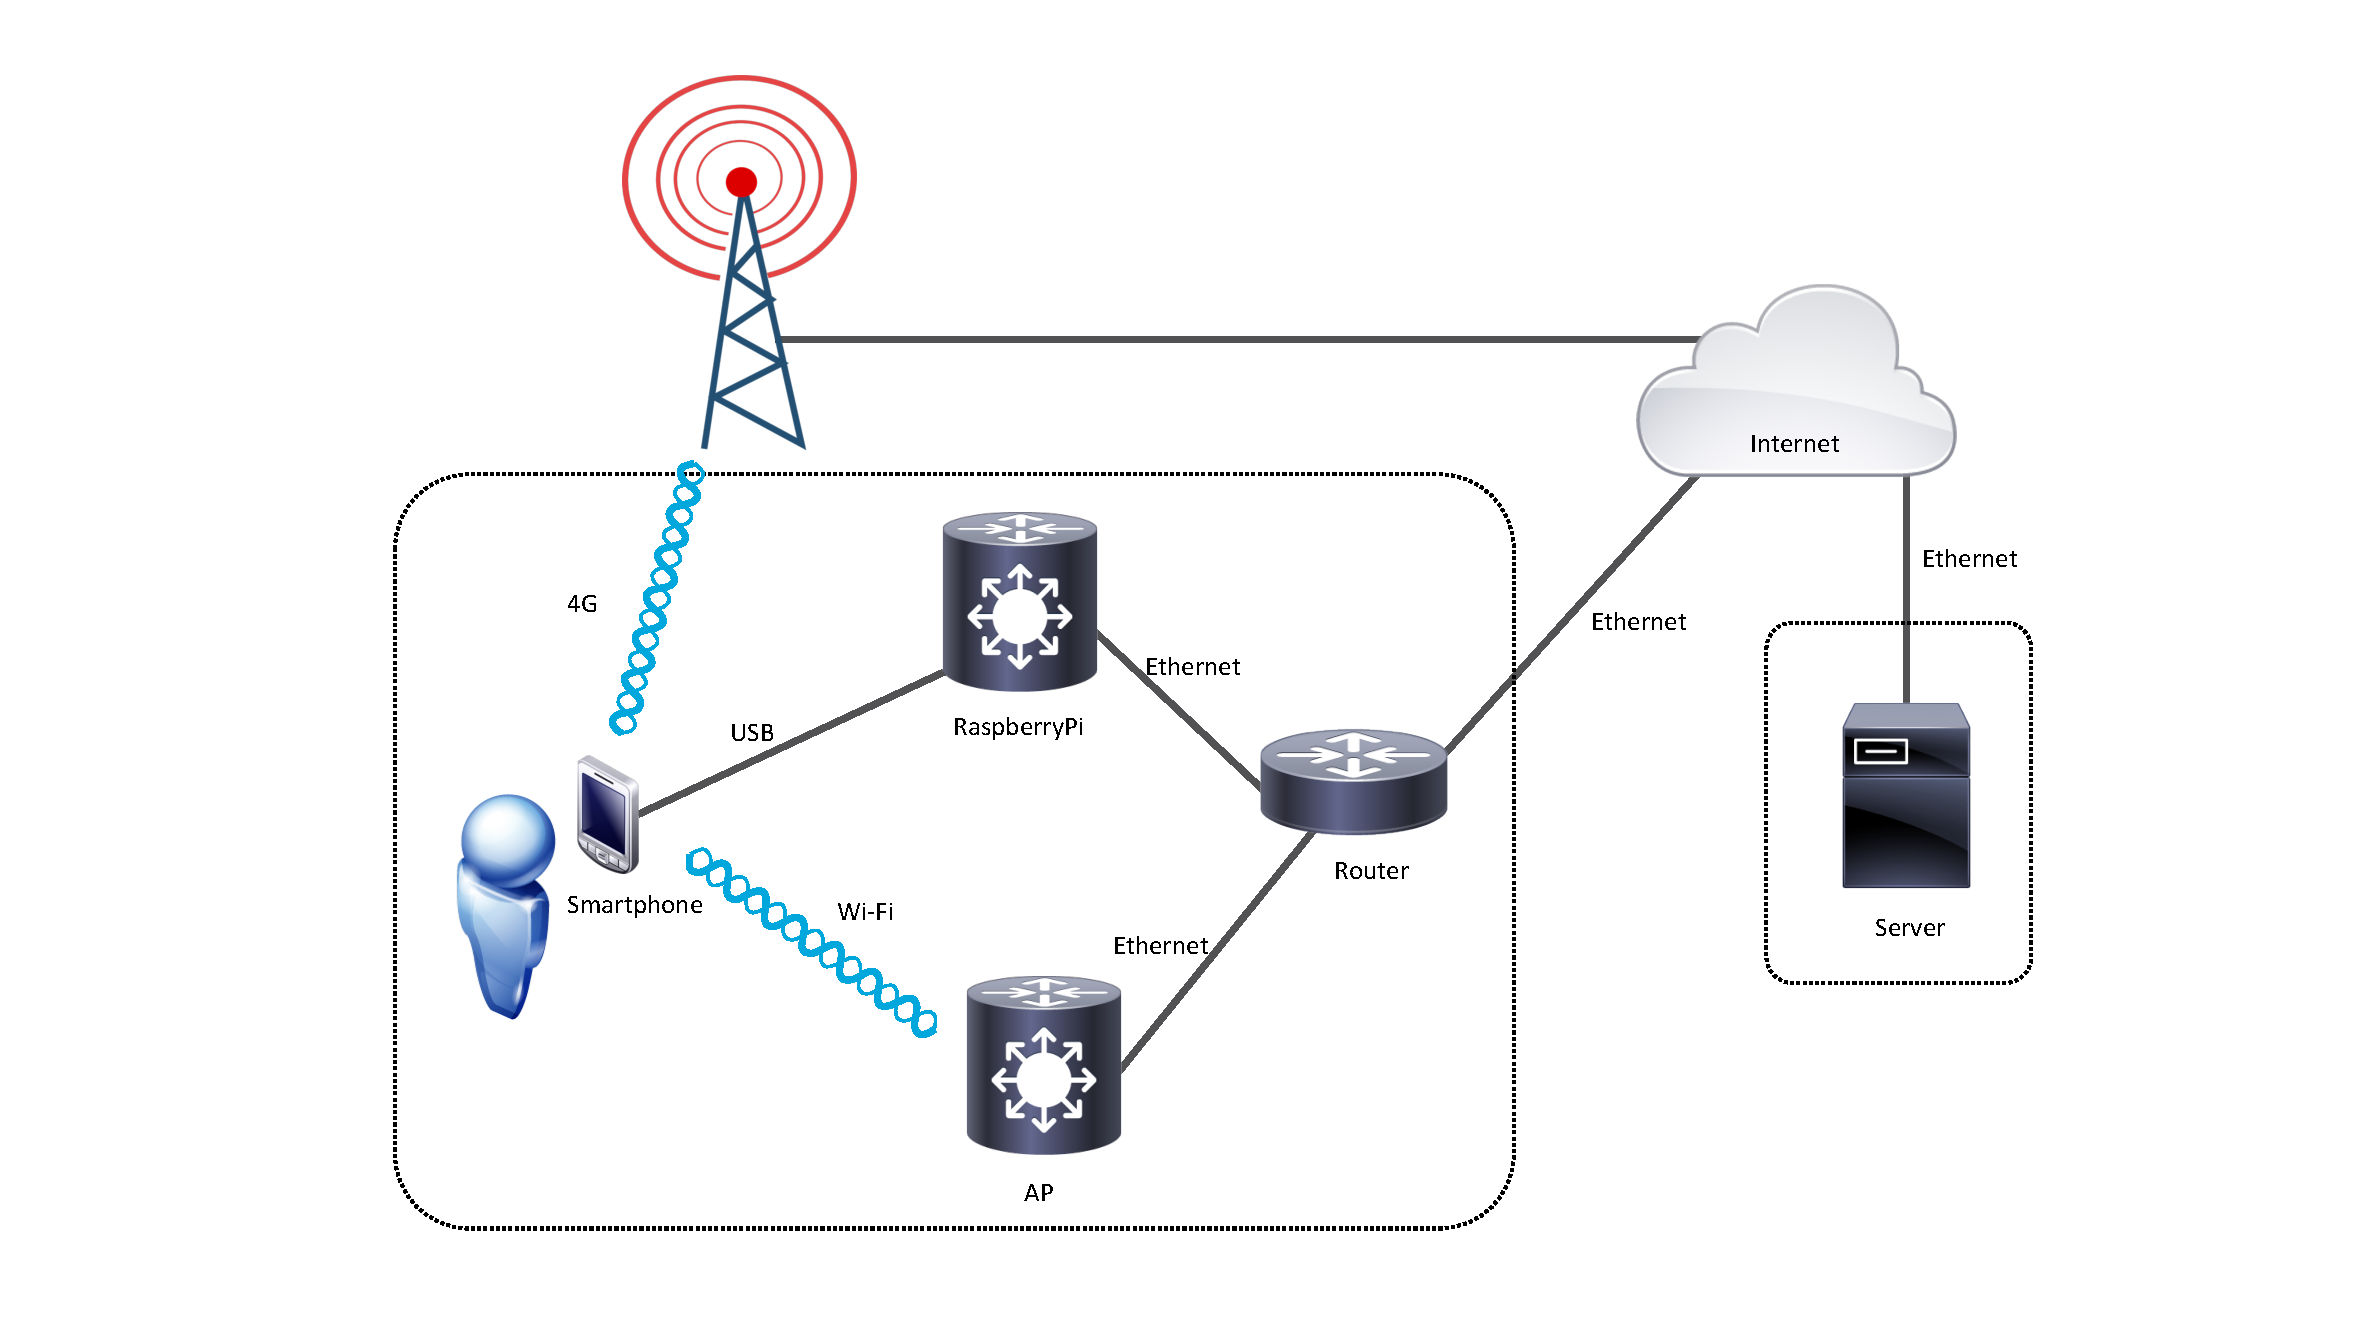
\includegraphics[scale=0.45]{figures/experiments/45G_Topology.pdf} 
	\caption{Arhitectura de test}
	\label{fig:topologie}
\end{figure}

\subsection{Determinarea zonei gri}

În scenariul considerat, un utilizator cu un telefon pornește de lângă AP-ul WiFi și se îndepărtează până când telefonul se deconectează de la WiFi. S-a simulat ieșirea din raza de acoperire a AP-ului prin scăderea puterilor acestuia, de la cea mai mare la cea mai mică. 

S-a realizat un experiment pentru determinarea zonei gri. Zona gri este definită de acele puteri ale AP-ului pentru care performanța este scăzută dar WiFi-ul rămâne conectat. Considerăm că MPTCP nu este activat (setare implicită).

Pentru evaluarea performanței s-a folosit scriptul \texttt{tcp\_ping} cu opțiunea \texttt{-datartt}, care înregistrează RTT-ul între telefon și serverul remote. 

Experimentul a fost executat prin implementarea unui script Python ce rulează pe RaspberryPi, care interacționează cu telefonul prin ADB și cu AP-ul prin SSH. Pașii realizați sunt următorii:
\begin{enumerate}
	\item Se setează puterea maximă, 17,  a AP-ului
	\item Se așteaptă evenimentul de conectare la WiFi a telefonului
	\item Se crează un thread care pornește scriptul \texttt{tcp\_ping} pe telefon, până se primește ultimul răspuns de la server și conexiunea cu serverul se închide
	\item Pe thread-ul principal, la fiecare 20 de secunde se scade cu o unitate puterea AP-ului până ajunge la 1
	\item Se realizează statistici legate de RTT pentru fiecare interval de 20 secunde
	\item Se memorează puterea AP-ului din momentul în care s-a închis conexiunea cu serverul 
\end{enumerate}

A fost rulat acest experiment de 50 de ori.

\subsection{Determinarea timpului mort și a timpului de start}

În al doilea rând s-a realizat un experiment pentru determinarea timpului mort în cadrul zonei gri. Acest timp mort este perioada de la ultimul răspuns de la server, până în momentul când telefonul se deconectează de la WiFi. În această perioadă WiFi-ul rămâne conectat chiar dacă telefonul nu mai poate comunica cu serverul (în loc să se decontecteze de la WiFi pentru a folosi 4G pentru comunicația cu serverul). Similar cu experimentul anterior, considerăm ca MPTCP nu este activat.

Timpul de start este perioada de la configurarea AP-ului pe puterea maximă , până în momentul când telefonul se conectează la WiFi. În acest timp telefonul folosește conexiunea 4G, chiar dacă pe WiFi ar putea avea o performanță mai bună (RTT mai mic).

Măsurarea timpului mort și a timpului de start s-a făcut folosind două configurații ale telefonului, cu următoarele opțiuni activate 1) WiFi, 4G, mobile data always on; 2) WiFi, 4G, mobile data always on, aggressive handover. 

Experimentul a fost orchestrat folosind un script Python rulat pe RaspberryPi. Acesta a interacționat cu telefonul prin ADB și cu AP-ul prin SSH. Figura \ref{fig:expdesign} reprezintă modul de desfășurare al experimentului. 

\begin{figure}[h!]
	\centering
	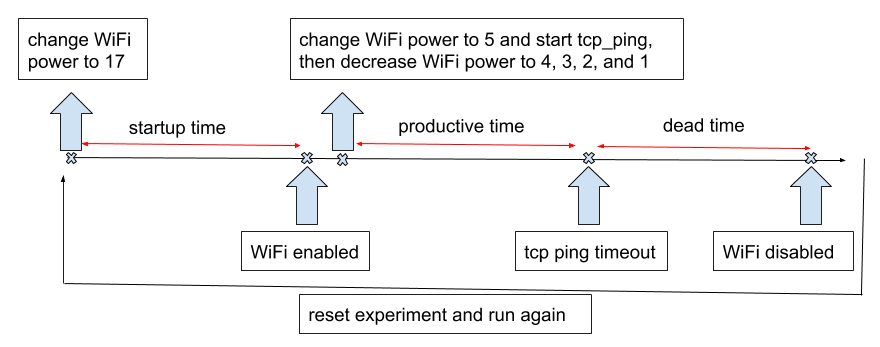
\includegraphics[scale=0.5]{figures/experiments/experiment_design.png}
	\caption{Modul de desfășurare al experimentului}
    	\label{fig:expdesign}
\end{figure}

Mai exact pașii realizați în cadrul experimentului sunt:
\begin{enumerate}
	\item Se setează puterea maximă, 17,  a AP-ului; se memorează timestamp-ul asociat (\texttt{start\_time})
	\item Se așteaptă evenimentul de conectare la WiFi pe telefon și se memorează timestamp-ului asociat evenimentului (\texttt{wifi\_enabled\_time})
	\item Dacă durează mai mult de 15 minute conectarea la WiFi, se resetează experimentul
	\item Se setează puterea 5 a AP-ului
	\item Se crează un thread care pornește scriptul \texttt{tcp\_ping} pe telefon, până se primește ultimul răspuns de la server și conexiunea cu serverul se închide; se memorează timestamp-ul asociat cu ultimul răspuns al serverului (\texttt{last\_reply\_time})
	\item După 20 de secunde se setează puterea 4 a AP-ului
	\item După 20 de secunde se setează puterea 3 a AP-ului
	\item După 20 de secunde se setează puterea 2 a AP-ului
	\item După 20 de secunde se setează puterea 1 a AP-ului
	\item Se așteaptă evenimentul de deconectare de la WiFi pe telefon, și se memorează timestamp-ul asociat evenimentului (\texttt{wifi\_disabled\_time})
	\item Dacă durează mai mult de 15 minute deconectarea de la WiFi, se resetează experimentul
	\item Se calculează \texttt{startup\_time = wifi\_enabled\_time - start\_time}
	\item Se calculează \texttt{productive\_time = last\_reply\_time - wifi\_enabled\_time}
	\item Se calculează \texttt{dead\_time = wifi\_disabled\_time - last\_reply\_time}
	\item Se reia experimentul (de 1000 ori)
\end{enumerate}

Evenimentele de conectare și deconectare a telefonului la WiFi sunt preluate prin ADB, din logurile generate în timp real de către aplicația ConnectivityMonitor. Astfel obținem în timp real aceste evenimente, cu timestamp-ul asociat.

Scriptul tcp\_ping este rulat de pe telefon, iar pornirea lui se face prin ADB. Output-ul script-ului conține asocieri între RTT-uri și timestamp-uri. Comenzile de schimbare a puterii AP-ului sunt date prin SSH către dispozitiv și returnează timestamp-ul asociat execuției comenzii pe AP. Pentru a obține niște perioade de timp corecte, ceasurile dispozitivelor sunt sincronizate.

S-a decis ca timpul maxim de așteptare a conectării și deconectării la WiFi să fie de 15 minute, deoarece un interval mai mare afectează foarte mult calitatea experienței utilizatorului. În aceste cazuri excepționale se resetează experimentul.

Un experiment conține 1000 de execuții ale pașilor de mai sus. S-au rulat 6 experimente: 3 fără și 3 cu aggresive handover. În urma acestor experimente s-a analizat timpul de startup și timpul mort.

\subsection{Handoff-ul în cazul folosirii MPTCP}

Acest experiment urmărește evaluarea handoff-ului în cazul folosirii MPTCP. A fost activat MPTCP folosind ConnectivityMonitor și au fost efectuați următorii pași:
\begin{enumerate}
	\item Se setează puterea maximă, 17,  a AP-ului
	\item Se așteaptă evenimentul de conectare la WiFi pe telefon
	\item Se crează un thread care pornește scriptul \texttt{tcp\_ping} pe telefon, până se primește ultimul răspuns de la server și conexiunea cu serverul se închide
	\item La fiecare 20 de secunde se scade cu o unitate puterea AP-ului până ajunge la 1.
	\item Se realizează statistici legate de RTT pentru fiecare interval de 20 secunde
\end{enumerate}

\section{Rezultate măsurători}

\subsection{Determinarea zonei gri}

În urma acestui experiment s-a observat că începând de la puterea 5 a AP-ului crește valoarea mediană a RTT-ului, iar la puterea 4 în cele mai multe cazuri se deconectează de la WiFi. Într-un număr redus de cazuri, telefonul se deconectează de la WiFi la puterile 3, 2 sau 1 ale AP-ului. În general valoarea mediană a RTT-ului crește considerabil atunci când AP-ul este configurat cu cele mai reduse puteri (4, 3, 2, 1), după cum se poate observa în exemplul de experiment din Listarea \ref{lst:zonagri}.

\lstdefinestyle{base}{
  emptylines=1,
  breaklines=true,
  basicstyle=\footnotesize\ttfamily\color{black},
  moredelim=**[is][\color{red}]{@}{@},
}

\begin{lstlisting}[label={lst:zonagri}, caption=Exemplu de zona gri, frame=single, style=base]
Power 17: mean=10.362 median=8.268 std=14.803 min=4.967 max=119.018
Power 16: mean=8.014 median=8.256 std=1.007 min=4.854 max=11.453
Power 15: mean=9.734 median=8.290 std=10.944 min=5.799 max=122.185
Power 14: mean=8.280 median=8.214 std=3.037 min=5.029 max=39.662
Power 13: mean=7.937 median=8.202 std=0.918 min=5.172 max=10.274
Power 12: mean=8.186 median=8.204 std=0.743 min=5.716 max=11.171
Power 11: mean=10.853 median=8.211 std=16.642 min=4.567 max=120.774
Power 10: mean=9.694 median=8.288 std=11.297 min=5.018 max=119.296
Power 9: mean=9.094 median=8.245 std=4.773 min=5.246 max=42.271
Power 8: mean=9.095 median=8.298 std=9.247 min=4.852 max=107.837
Power 7: mean=8.136 median=8.249 std=1.051 min=4.992 max=12.477
Power 6: mean=12.593 median=8.269 std=21.592 min=4.796 max=123.357
@Power 5: mean=15.070 median=8.264 std=42.867 min=5.170 max=443.009
Power 4: mean=2179.825 median=120.305 std=3510.848 min=7.434 max=15716.309
Power 3: mean=8910.837 median=6422.250 std=7904.022 min=125.882 max=23084.616
Power 2: mean=3812.544 median=126.536 std=7506.864 min=15.716 max=31130.847
Power 1: mean=5960.073 median=2659.242 std=6958.977 min=113.620 max=18298.263
@
\end{lstlisting}

Prin urmare, considerăm zona gri, acea perioadă în care AP-ul are puteri între 5 și 1. Această zonă simulează ieșirea utilizatorului din raza de acoperire a AP-ului, în care deși telefonul este conectat la WiFi, performanța este foarte scăzută. 

În continuare, s-a folosit acest interval de puteri ale AP-ului pentru a determina timpul mort și timpul de startup.

\subsection{Determinarea timpului mort și a timpului de startup}

\subsubsection{Configurația fără aggresive handover}

În Figura \ref{fig:deadtime1} este reprezentată distribuția timpului mort în intervalele 0-10, 10-20, 20-30, 30-40 și 40-900 secunde, în cazul configurației fără aggressive handover, în cadrul a trei experimente distincte. 

Observăm că cele mai multe valori sunt în intervalul 10-20 secunde, iar medianele sunt de 14, 12 și 14 secunde. De asemenea, este important faptul că apar un număr considerabil de valori în intervalul 40-900 secunde, timp în care conexiunea cu serverul nu funcționează, ceea ce duce la reducerea calității experienței utilizatorului. 

\begin{figure*}[h!]
$\begin{array}{rl}
    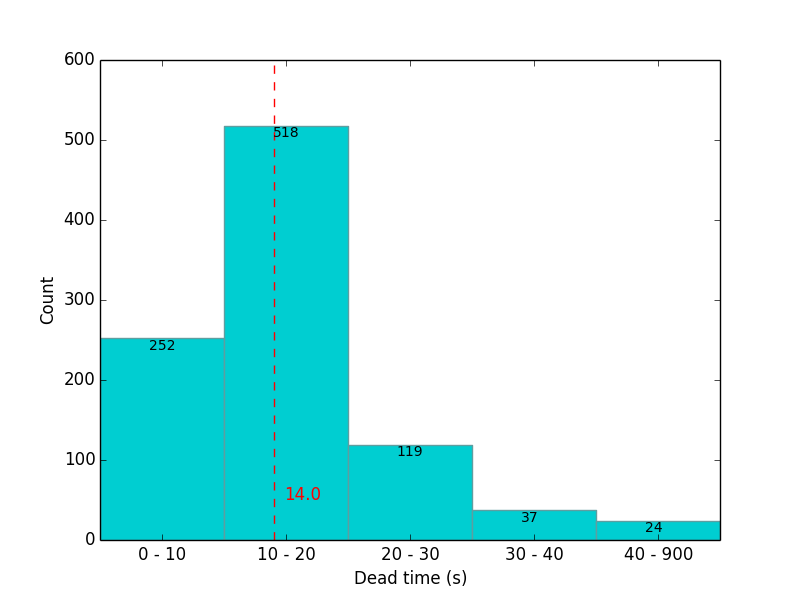
\includegraphics[width=0.5\textwidth]{figures/experiments/dead_time23.png} &
    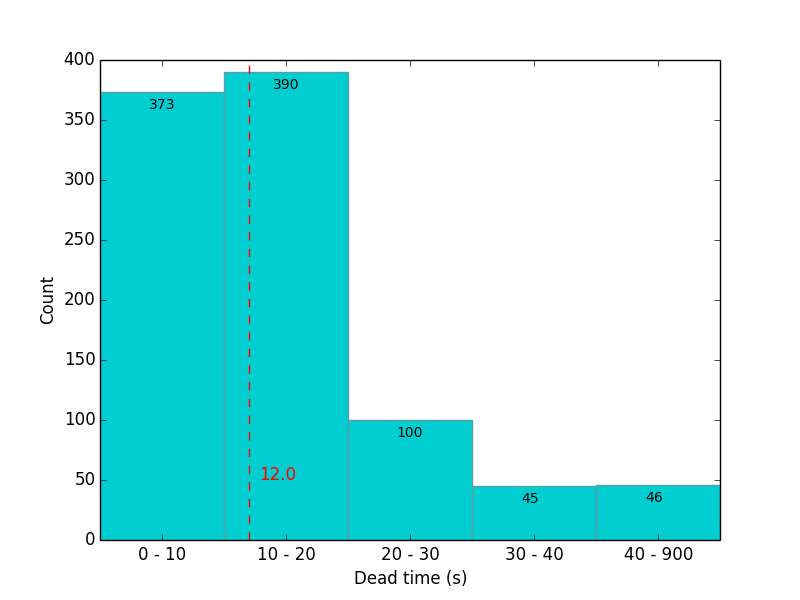
\includegraphics[width=0.5\textwidth]{figures/experiments/dead_time25.png}\\
    \multicolumn{2}{c}{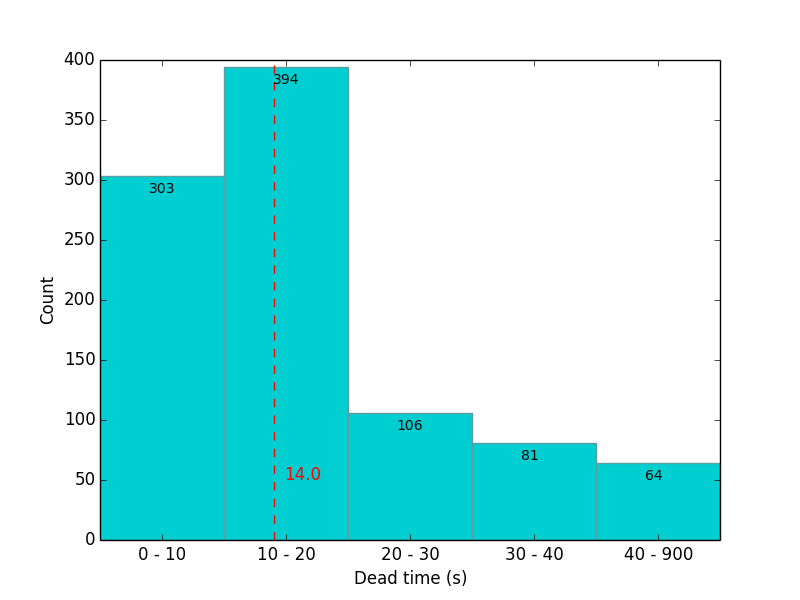
\includegraphics[width=0.5\textwidth]{figures/experiments/dead_time27.png}}
\end{array}$
\caption{Timp mort - configurația fără aggresive handover}
\label{fig:deadtime1}
\end{figure*}

În Figura \ref{fig:startuptime1} este reprezentată distribuția timpului de startup în intervalele 0-10, 10-20, 20-30, 30-40 și 40-900 secunde, în exact aceleași experimente menționate anterior. 

Deși distribuția este diferită în cadrul celor 3 experimente, observăm că medianele sunt apropiate: 28, 32, 27 secunde. Observăm un număr destul de mare de valori în intervalul 40-900 secunde, ceea ce afectează experiența utilizatorului, care va folosi 4G in loc de WiFi, chiar dacă este disponibil cu putere maximă.

\begin{figure*}[h!]
$\begin{array}{rl}
    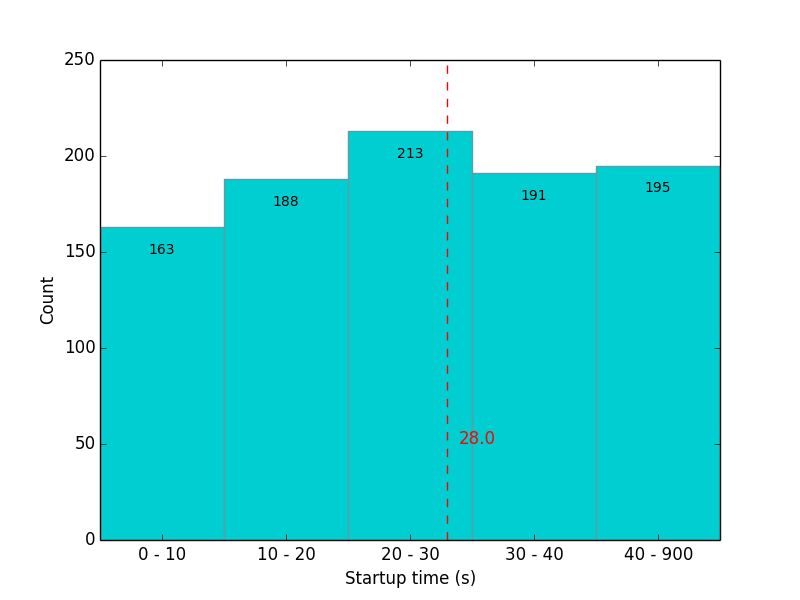
\includegraphics[width=0.5\textwidth]{figures/experiments/startup_time23.png} &
    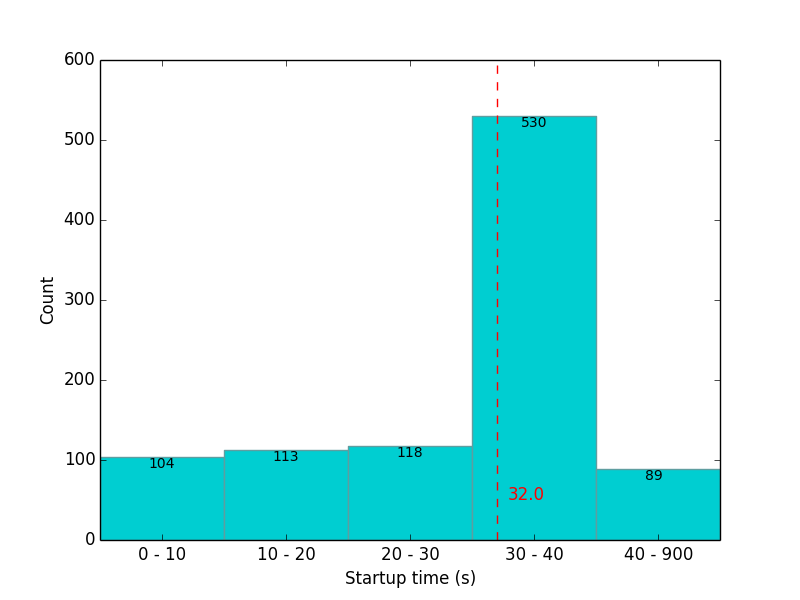
\includegraphics[width=0.5\textwidth]{figures/experiments/startup_time25.png}\\
    \multicolumn{2}{c}{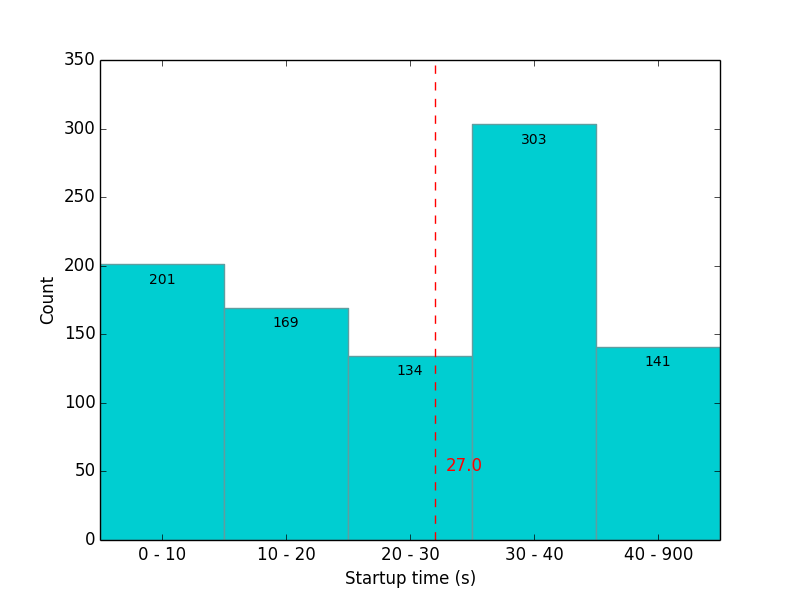
\includegraphics[width=0.5\textwidth]{figures/experiments/startup_time27.png}}
\end{array}$
\caption{Timp de startup - configurația fără aggresive handover}
\label{fig:startuptime1}
\end{figure*}

\subsubsection{Configurația cu aggresive handover}

În această secțiune sunt prezentate rezultatele experimentelor rulate cu configurația aggresive handover. În Figura \ref{fig:deadtime2}, este reprezentată distribuția timpului mort în intervalele 0-10, 10-20, 20-30, 30-40 și 40-900 secunde, în trei experimente distincte.

Putem observa că rezultatele sunt similare față de configurația anterioară (fără aggressive handover). Cele mai multe valori se găsesc în intervalul 10-20 secunde, iar medianele sunt similare: 14, 14, 13. 

Mai putem determina faptul că avem mai multe valori în intervalul 40-900 față de configurația anterioară. Acest lucru ne arată faptul că această configurație nu ajută în micșorarea timpului mort. 

\begin{figure*}[h!]
$\begin{array}{rl}
    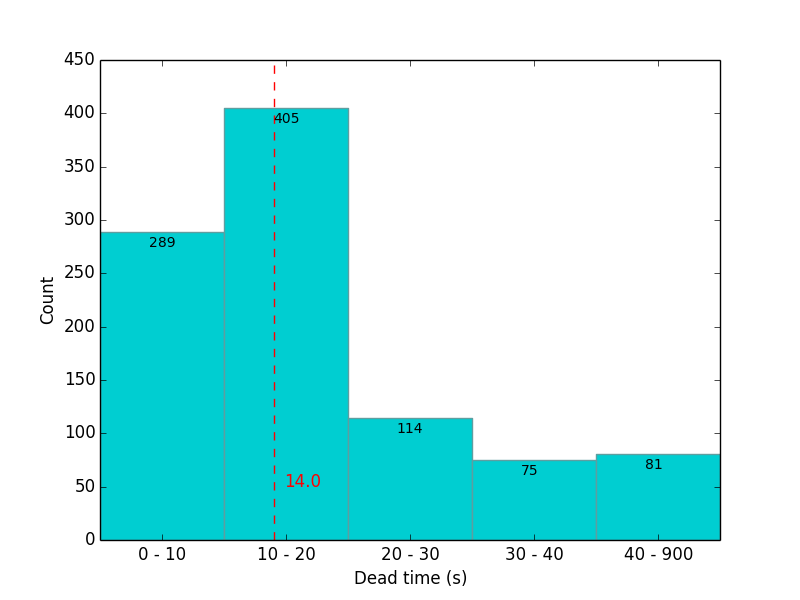
\includegraphics[width=0.5\textwidth]{figures/experiments/dead_time30.png} &
    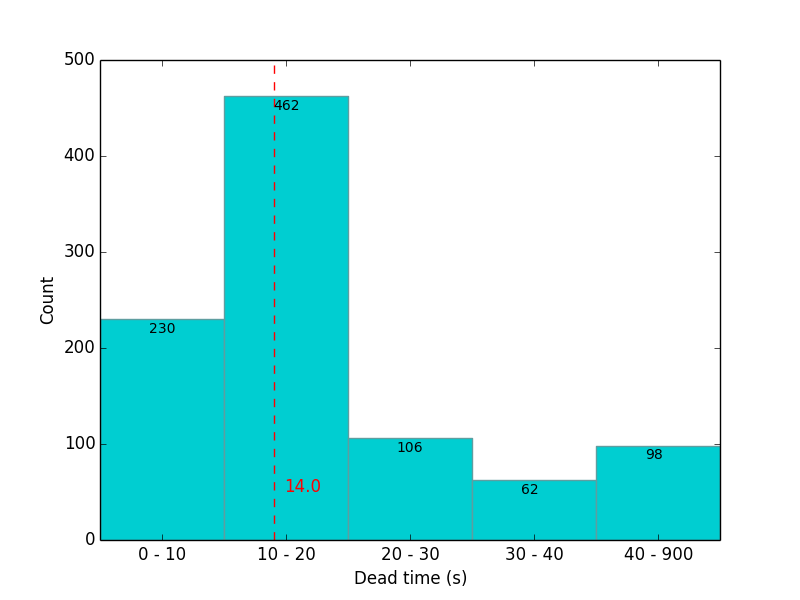
\includegraphics[width=0.5\textwidth]{figures/experiments/dead_time31.png}\\
    \multicolumn{2}{c}{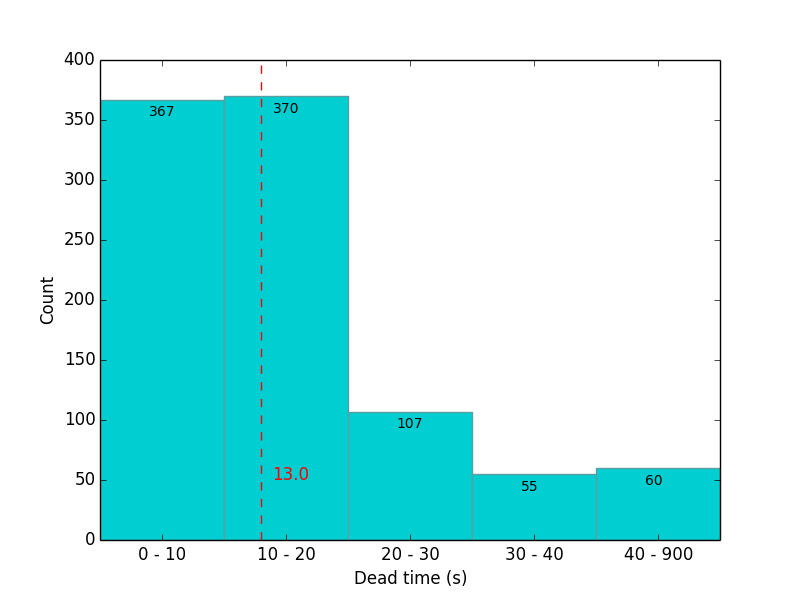
\includegraphics[width=0.5\textwidth]{figures/experiments/dead_time32.png}}
\end{array}$
\caption{Timp mort - configurația cu aggresive handover}
\label{fig:deadtime2}
\end{figure*}

În Figura \ref{fig:startuptime2} este reprezentată distribuția timpului de startup în intervalele 0-10, 10-20, 20-30, 30-40 și 40-900 secunde, în experimentele menționate anterior. 

Observăm că medianele sunt similare între ele și asemănătoare cu cele de la experimentele cu configurația anterioară: 29.5, 24, 29. Un număr mare de valori rămâne în intervalul 40-900 secunde, afectând experiența utilizatorului.

\begin{figure*}[h!]
$\begin{array}{rl}
    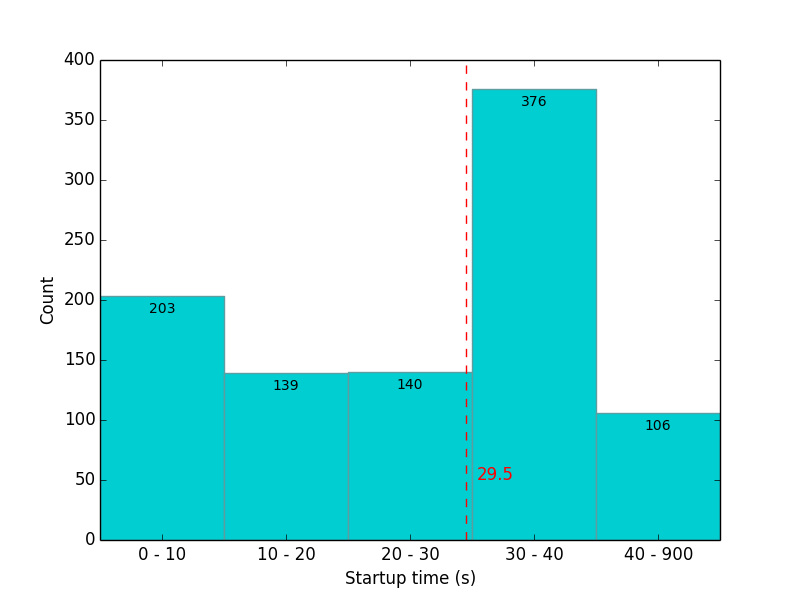
\includegraphics[width=0.5\textwidth]{figures/experiments/startup_time30.png} &
    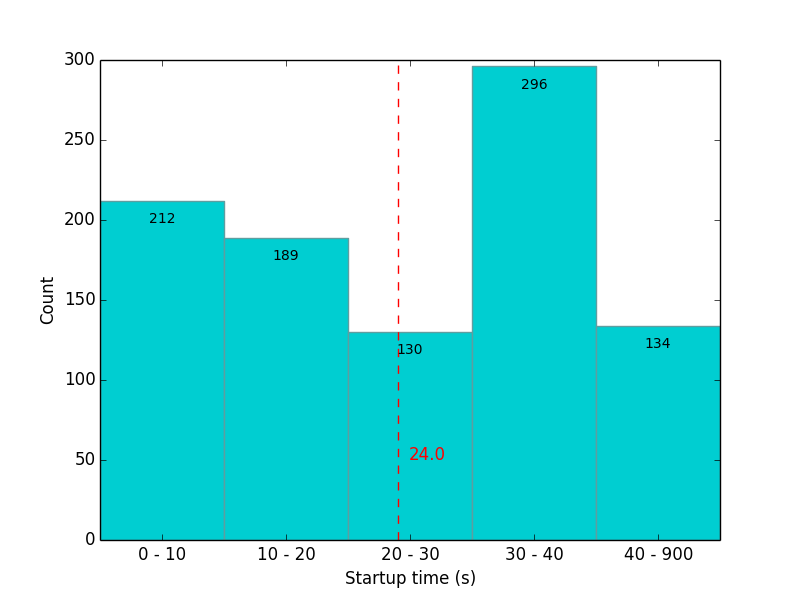
\includegraphics[width=0.5\textwidth]{figures/experiments/startup_time31.png}\\
    \multicolumn{2}{c}{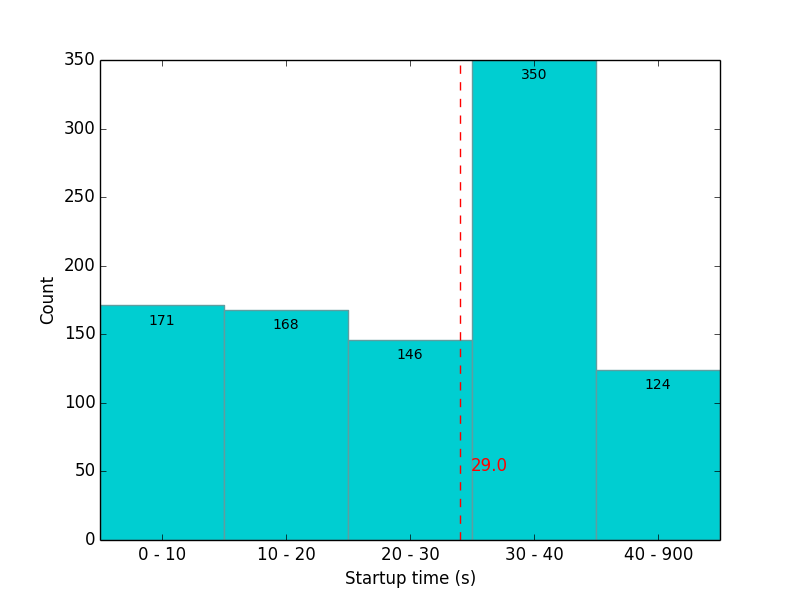
\includegraphics[width=0.5\textwidth]{figures/experiments/startup_time32.png}}
\end{array}$
\caption{Timp de startup - configurația fără aggresive handover}
\label{fig:startuptime2}
\end{figure*}

Valorile ridicate ale timpului mort în ambele configurații, demonstrează faptul că fără MPTCP, telefonul își va pierde conexiunile existente atunci când se îndepărtează de AP (când puterea AP-ului scade), și va rămâne o perioadă fără conexiune funcțională la Internet, chiar dacă rețeaua 4G era disponibilă. 

\subsubsection{Alte rezultate}

Pentru cele 6 experimente (cu câte 1000 de rulări fiecare), timpul maxim de așteptare a evenimentelor de conectare și deconectare de la WiFi a fost setat la 15 minute. Depășirea acestui timp la conectare/deconectare pe WiFi duce la restarea experimentului deoarece ar afecta prea mult experiența utilizatorului.

Tabelul \ref{tab:timeout} include pentru fiecare experiment numărul de resetări datorate timeout-ului la conectare, la deconectare și numărul total de resetări. Observăm ca numărul total de resetări în cazul experimentelor 4,5,6 este ușor mai scăzut decât în cazul experimentelor 1,2,3. Înafară de acest lucru, nu se poate observa o diferență notabilă între cele două configurații.

\begin{table}[h!]
\centering
\caption{Timeout la conectare/deconectare WiFi}
\label{tab:timeout}
\begin{tabular}{c | c | p{3cm} | p{3cm} | p{2cm}}
\hline
Experiment & Aggresive handover& Resetări datorate timeout-ului la conectare & Resetări datorate timeout-ului la deconectare  & Număr total de resetări \\
\hline
1 & dezactivat & 45 & 6 & 51 \\
2 & dezactivat & 25 & 22 & 47 \\
3 & dezactivat & 28 & 25 & 53 \\
4 & activat  & 35 & 2 & 37 \\
5 & activat & 28 & 12& 40 \\
6 & activat & 17 & 25 & 42 \\
\hline
\end{tabular}
\end{table}

Alt rezultat extras din cele 6 experimente este puterea la care a fost primit ultimul răspuns din partea serverului. Tabelul \ref{tab:putere} include pentru fiecare experiment numărul de iterații asociate cu fiecare putere a AP-ului (la care s-a primit ultimul răspuns de la server).

\begin{table}[h!]
\centering
\caption{Puterea AP-ului asociată ultimului răspuns de la server}
\label{tab:putere}
\begin{tabular}{c | c | c | c | c | c | c}
\hline
Experiment & Aggresive handover& Puterea 5 & Puterea 4 & Puterea 3 & Puterea 2 & Puterea 1 \\
\hline
1 & dezactivat & 747 & 154 & 11 & 7 & 29 \\
2 & dezactivat & 50 & 867 & 11 & 2 & 45 \\
3 & dezactivat & 368 & 492 & 24 & 11 & 72 \\
4 & activat  & 813 & 65 & 8 & 8 & 59 \\
5 & activat  & 810 & 74 & 16 & 9 & 62 \\
6 & activat  & 525 & 362 & 16 & 7 & 73 \\
\hline
\end{tabular}
\end{table}

\subsection{Handoff-ul în cazul folosirii MPTCP}

În urma acestui experiment s-a observat faptul că conexiunea cu serverul este continuă, nu se închide atunci când puterea AP-ului scade, deoarece traficul este preluat de către al doilea flow, cel care folosește conexiunea 4G. Acest lucru este realizat înainte de a se ajunge la RTT-uri foarte mari (puteri mici ale AP-ului). Prin urmare, performanța este menținută chiar dacă se iese din raza de acoperire a AP-ului.

Astfel, folosirea MPTCP ne asigură păstrarea conexiunilor existente și menținerea performanței (RTT-ul nu scade mult sub cel al conexiunii 4G).
